
\documentclass{article}
\usepackage{aligned-overset}
\usepackage{amsmath}
\usepackage{amssymb}
\usepackage{bm}
\usepackage[shortlabels]{enumitem}
\usepackage{hyperref}
\usepackage[utf8]{inputenc}
\usepackage{mathtools}
\usepackage{physics}
\usepackage{tabularx}
\usepackage{titling}
\usepackage{fancyhdr}
\usepackage{xfrac}
\usepackage{pgfplots}

\definecolor{light-gray}{gray}{.9}

\pgfplotsset{compat = newest}
\usetikzlibrary{intersections}
\usetikzlibrary{patterns}
\usepgfplotslibrary{fillbetween}

\author{Karsten Lehmann}
\date{SoSe 2021}
\title{Übung 04 Analysis - Weiterführende Konzepte}

\pagestyle{fancy}
\fancyhf{}
\lhead{\thetitle}
\rhead{\theauthor}
\lfoot{\thedate}
\rfoot{Seite \thepage}

\begin{document}

\section*{Räume stetiger und differenzierbarer Funktionen}

Wir betrachten den Vektorraum $C[0, 1]$ der stetigen Funktionen auf dem
Intervall $[0, 1]$.
Für $f \in C[0, 1]$ definieren wir die \textit{Supremumsnorm} durch
\[
  \norm{f}_{\infty} \coloneqq \sup\qty{\abs{f(x)} \middle| x \in [0, 1]}
\]

\textit{Lsg.} $C([0, 1]) = \qty{f \colon [0, 1] \to \mathbb{R} \middle| \,\text{$f$ ist stetig}}$ ist ein Vektorraum.
  \begin{align*}
    (f + g)(x) &\coloneqq f(x) + g(x) \\
    (\lambda \cdot f)(x) &\coloneqq \lambda \cdot f(x)
  \end{align*}
  Die Dimension von $C([0, 1])$ ist unendlich, da
  $f_n(x) \coloneqq x^n, n \in \mathbb{N}$
  Jedes Teilsystem $\qty{f_{n_1}, \ldots, f_{n_k}}$ besteht aus linear unabhängigen Funktionen.

  \[
    \underset{\lambda_0 = \lambda_1 = \ldots = \lambda_n = 0}{\underset{\Updownarrow}{\underbrace{\sum_{k = 0}^n \lambda_k f_k}}} = 0
    \underset{\iff \lambda_0 = \lambda_1 = \ldots = \lambda_n = 0}{\iff \sum_{k = 0}^n \lambda_k f_k(x) = 0} \text{ für alle } x \in [0, 1]
  \]

\begin{enumerate}[(i)]
\item Ermitteln Sie $\norm{f_k}_{\infty}$ für $f_1(x) \coloneqq \sin(2\pi x)$,
  $f_2(x) \coloneqq x(1 - x)$, $f_3(x) \coloneqq (x + 1)(2x - 1)$.

  \textit{Lsg.} Ermittlung lokaler Extrema:
  \begin{enumerate}[1)]
  \item $f_1'(x) = 2 \pi \cos(2\pi x)$

    $f_1'(x) = 0, x \in [0, 1] \iff x_1 = \sfrac{1}{4}, x_2 = \sfrac{3}{4}$

    $\norm{f_1}_{\infty} = \max\qty{\abs{f_1(0)}, \abs{f_1(\sfrac{1}{4})}, \abs{f_1(\sfrac{3}{4})}, \abs{f_1(1}} = 1$

  \item $f_2'(x) = -2x + 1$

    $f_2'(x) = 0, x \in [0, 1] \iff x = \sfrac{1}{2}$

    $\norm{f_2}_{\infty} = \max\qty{\abs{f_2(0)}, \abs{f_2(\sfrac{1}{2})}, \abs{f_2(1}} = \sfrac{1}{4}$

  \item $f_3'(x) = 4x + 1$

    $f_3'(x) = 0, x \in [0, 1] \iff x = -\sfrac{1}{4}$ und $-\sfrac{1}{4}$ ist nicht im Intervall $[0, 1]$ enthalten.

    $\norm{f_3}_{\infty} = \max\qty{\abs{f_3(0)}, \abs{f_3(1}} = 2$
  \end{enumerate}

\newpage
\item Zeigen Sie, dass $(C([0, 1]), \norm{\cdot}_{\infty})$ ein normierter Raum ist.

  \textit{Lsg.}
  \begin{itemize}
  \item $\norm{f}_{\infty} = \underset{x \in [0, 1]}{\sup \abs{f(x)}}
    \overset{\text{Satz von Bolzano-Weierstraß}}{< +\infty}$
  \item $\norm{f}_{\infty} \geq \abs{f(0)} > 0 \,\forall f \in C([0, 1])$
  \item $\norm{f}_{\infty} = 0 \iff \underset{x \in [0, 1]}{\sup} \abs{f(x)} \iff \abs{f(x)} = 0
    \,\forall x \in [0, 1] \iff f = 0$
  \item $\forall \lambda \in \mathbb{R}, f \in C([0, 1]) \colon
    \norm{\lambda f}_{\infty} = \underset{x \in [0, 1]}{\sup} \abs{\lambda f(x)}
    = \abs{\lambda} \underset{x \in [0, 1]}{\sup} \abs{f(x)} = \abs{\lambda} \norm{f}_{\infty}$
  \item Dreiecksungleichung: $\forall f, g \in C([0, 1])$ gilt:

    $\norm{f + g}_{\infty} = \underset{x \in [0, 1]}{\sup}
    \underset{\leq \underset{\leq \norm{f}_{\infty}}{\underbrace{\abs{f(x)}}} +
      \underset{\leq \norm{g}_{\infty}}{\underbrace{\abs{g(x)}}}}
    {\underbrace{\abs{f(x) + g(x)}}}
    \leq \norm{f}_{\infty} + \norm{g}_{\infty}$
  \end{itemize}

\item Beweisen Sie, dass $(C([0, 1]), \norm{\cdot}_{\infty})$ vollständig ist.

  \textit{Lsg.} Sei $\qty(f_n)$ eine Cauchy-Folge, d.h.
  \[
    \forall \epsilon > 0 \,\exists n_0 \in \mathbb{N} \forall m, n > n_0 \colon \norm{f_n - f_m}
    = \underset{x \in [0, 1]}{\sup} \abs{f_n(x) - f_m(x)} < \epsilon
  \]
  $\Rightarrow$ Für alle $x \in [0, 1]$ gilt $\abs{f_n(x) - f_m(x)} < \epsilon$ für alle $m, n \geq n_0$

  $\Rightarrow$ Für alle $x \in [0, 1]$ ist $\qty(f_n(x))_{n \in \mathbb{N}}$ eine Cauchy-Folge.

  Da $(\mathbb{R}, \abs{\cdot})$ vollständig ist, existiert der Punktweise Grenzwert
  $f(x) \coloneqq \lim_{n \to \infty} f_n(x)$ für alle $x \in [0, 1]$.

  Da $\qty(f_n)$ eine Cauchy-Folge ist existiert für alle $\epsilon > 0$ ein $n_0 \in \mathbb{N}$
  mit $\norm{f_n - f_m}_{\infty} < \frac{\epsilon}{2}$ für alle $m, n \geq n_0$.

  Für $x \in [0, 1]$ folgt für $n > n_0$
  \[
    \lim_{m \to \infty} \abs{f_n(x) - f_m(x)} = \abs{f_n(x) - f(x)} \leq \frac{\epsilon}{2}
  \]

  $\Rightarrow \norm{f_{n_0} - f}_{\infty} =
  \underset{x \in [0, 1]}{\sup} \abs{f_{n_0} (x) - f()x}
  \leq \frac{\epsilon}{2}$

  Für $n \geq n_0$ ergibt sich
  \[
    \norm{f_n - f}_{\infty} \leq \underset{< \frac{\epsilon}{2}}{\underbrace{\norm{f_n - f_{n_0}}_{\infty}}} +
    \underset{\leq \frac{\epsilon}{2}}{\underbrace{\norm{f_{n_0} - f}_{\infty}}} < \epsilon
  \]

  $\Rightarrow f_n \overset{n \to \infty}{\longrightarrow} f$ bezüglich $\norm{\cdot}_{\infty}$ (Gleichmäßige Konvergen z)

  $f \in C([0, 1])$, wegen Theorem 3.4.2 der Vorlesung (\textit{Gleichmäßige Limiten stetiger Funktionen sind stetig})
\end{enumerate}

\section*{Metrische Räume und induzierte Metrik}

Wir betrachten den normierten Raum $(\mathbb{R}^2, \norm{\cdot}_2)$.
Skizzieren Sie die folgenden Mengen $A \subseteq \mathbb{R}^2$ und untersuchen Sie,
ob diese offen, abgeschlossen bzw. Umgebungen des Nullpunktes sind.
Geben Sie jeweils das Innere $\mathring A$, den Abschluss $\overline{A}$,
den Rand $\partial A$ und die isolierten Punkte dieser Mengen an.

\textit{Lsg.} Sei $(M, d)$ ein metrischer Raum und $A \subseteq M$.

\begin{itemize}
\item $x \in \mathring A = \text{int} A \iff \exists r > 0 \colon B(x, r) \subseteq A$
\item $\mathring A$ ist die größte offene Teilmenge von $A$.
  $A \subseteq M$ heißt offen, falls $A = \mathring A$ gilt.

  $x \in \partial A \iff x \in \overline A \setminus \mathring A
  \iff \forall r > 0 \colon B(x, r) \cap A \ne \emptyset \land B(x, r) \cap (M \setminus A) \ne \emptyset$

  $\partial A = \partial (M \setminus A)$
\item $A \subseteq M$ heißt abgeschlossen $\iff M \setminus A$ ist offen.
  $\overline A$ Abschluss von $A \colon$ kleinste abgeschlossene Menge von $A$

  $x \in \overline A \iff \forall r > 0 \colon B(x, r) \cap A \ne \emptyset$

  Es gibt eine Folge $\qty(x_n)$ in $A$ mit $x_n \to x$
\end{itemize}

$x$ ist isolierter Punkt von $A \iff \exists r > 0 \colon B(x, r) \cap A = \qty{x})$

\begin{enumerate}[(i)]
\item $A = B(x, r)$ mit $x \in \mathbb{R}^2$ und $r > 0$

  \textit{Lsg.} $A = \mathring A \colon $ Sei $y \in B(x, r) \Rightarrow \epsilon = r - \norm{x - y}_2 > 0$

  Zu zeigen ist nun, dass $y \in \mathring A$:

  Es gilt $B(y, \epsilon) \subseteq B(x, r) \colon$ Sei $z \in B(y, \epsilon)$

  $\Rightarrow \norm{x - z}_2 \leq \norm{x - y}_2 + \underset{< \epsilon}{\underbrace{\norm{y - z}_2}}
  < \norm{x - y}_2 + (r - \norm{x - y}_2) = r$

  $\Rightarrow z \in B(x, r) \Rightarrow$ die Menge ist offen.

  Es gilt $\partial A = S(x, r) = \qty{ y \in \mathbb{R}^2 \middle| \norm{x - y}_2 = r }$

  Ist $\norm{x - y} > r$, dann existiert ein $\epsilon > 0$ mit
  $B(y, \epsilon) \subseteq \mathbb{R}_2 \setminus A$

  $\Rightarrow y$ ist kein Randpunkt von $A$ und gehört nicht zu $\mathring A$.

  $A = \mathring A \cup \partial A = B[x, r]$
\item $A = B[x, r] = \qty{y \in \mathbb{R}^2 \middle| \norm{x - y}_2 \leq r}$ mit $x \in \mathbb{R}^2$ und $r > 0$

  \textit{Lsg.} $A$ ist eine abgeschlossene Kugel, da $\overline A = A$ gilt.

  Weiter ist $\mathring A = B(x, r)$ und $\partial A = S(x, r)$

\item $A = \qty{y \in \mathbb{R}^2 \middle| \norm{x - y}_2 > r}$ mit $x \in \mathbb{R}^2$ und $r > 0$

  \textit{Lsg.} $A$ ist offen (da $\mathbb{R}^2$ ohne abgeschlossene Kugel), d.h. $A = \mathring A$

  $\partial A = \partial B[x, r] = S(x, r)$

  $\overline A = \qty{y \in \mathbb{R}^2 \middle| \norm{x - y}_2 \geq r}$

\item $A = \qty{x = \qty(x_1, x_2) \in \mathbb{R}^2 \middle| \qty(x_1 > -1) \land \qty(x_2 \geq -1)}$

  \textit{Lsg.}:

  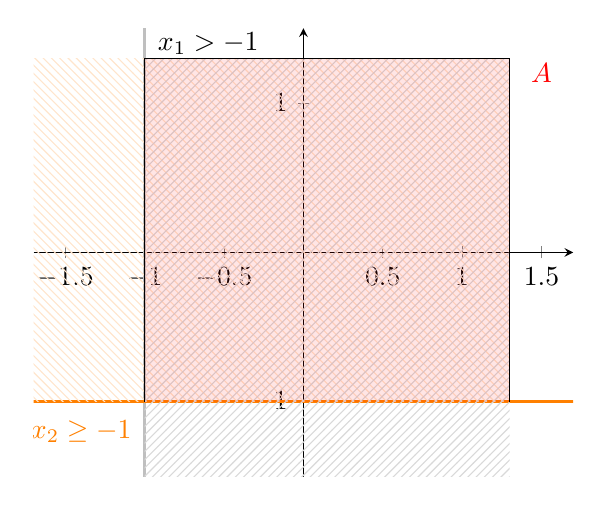
\begin{tikzpicture}
    \begin{axis}[
      axis lines=middle,
      xmax = 1.7,
      xmin = -1.7,
      ymax = 1.5,
      ymin = -1.5,]
      \addplot [
        name path=f,
        very thick,
        gray!50] coordinates {(-1,-2) (-1, 2)};
      \addplot [
        name path=g,
        domain=-2:2,
        samples=100,
        very thick, orange]{-1};
      \addplot[draw=none, pattern color=orange!20, pattern=north west lines] coordinates
        {(-2, 1.3) (1.3, 1.3) (1.3, -1) (-2, -1)};
      \addplot[draw=none, pattern color=gray!30, pattern=north east lines] coordinates
        {(-1, 1.3) (1.3, 1.3) (1.3, -2) (-1, -2)};
      \node[orange] at (-1.4, -1.2) {$x_2 \geq -1$};
      \node at (-0.6, 1.4) {$x_1 > -1$};
      \node[red] at (1.5, 1.2) {$A$};
      \addplot[fill=red, fill opacity=.1] coordinates {(-1,-1) (-1,1.3) (1.3,1.3) (1.3,-1)};
    \end{axis}
  \end{tikzpicture}

  $\mathring A = \qty{x = \qty(x_1, x_2) \middle| x_1 > -1 \land x_2 > -1 }$ (eine echte Teilmenge von $A$).

  $\partial A = \qty{ (-1, x_2), (x_1, -1) \middle| x_1, x_2 \geq 0 }$

  $\overline A = \mathring A \cup \partial A = \qty{x \in \mathbb{R}^2 \middle| x_1 \geq 0 \land x_2 \geq 0}$
  (eine echte Unmenge zu $A \Rightarrow A$ ist nicht abgeschlossen)

\item $A = \qty{ x_n = \qty(\frac{1}{n}, 0) \middle| n \in \mathbb{N}}$

  \textit{Lsg.}

    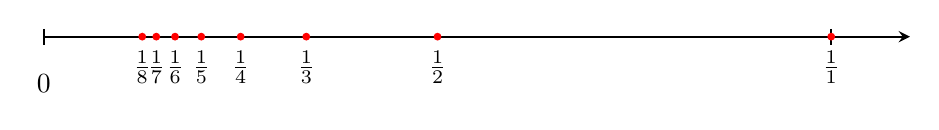
\begin{tikzpicture}
      \draw[-stealth, thick] (0,0) -> (11,0);
      \draw[thick] (0,.1) -- ++(0,-.2);
      \draw[thick] (10,.1) -- ++(0,-.2);
      \node at (0, -.6) {0};
      \foreach \x [evaluate=\x as \xx using (10/\x)]in {1,...,8} {
        \node[circle, fill=red, inner sep=1pt, label=below:$\frac{1}{\x}$] at (\xx, 0) {};
      }
  \end{tikzpicture}

  $\mathring A = \emptyset, \partial A = A \cup \qty{(0, 0)} \supsetneqq A$ wegen $\lim_{n \to \infty} x_n = 0$

  $\Rightarrow A$ ist weder offen noch abgeschlossen.

  Alle Punkte aus $A$ sind isoliert.
\end{enumerate}

\newpage
Wir betrachten den metrischen Raum $(\mathbb{R}, d)$ mit $d(x, y) = \abs{x - y}, x, y \in \mathbb{R}$.
Die Menge $M = [0, 1) \cup \qty{\frac{3}{2}} \cup(2, 3)$ sei mit der induzierten Metrik
$d_M \coloneqq d|_{M \times M}$ versehen, so dass der metrische Raum $\qty(M, d_M)$ entsteht.

\textit{Lsg.} Sei $(X, d)$ ein metrischer Raum und $M \subseteq X$ eine nichtleere Teilmenge von $X$.

$d_M \colon M \times M \to \mathbb{R}$ mit $d_m(x, y) \coloneqq d(x, y) \quad x, y \in M$
auf $M$ induzierte Metrik.

\begin{align*}
  B_d(x, r) &= \qty{ y \in X \middle| d(x, y) < r } \\
  B_{d_M}(x, r) &= \qty{ y \in M \middle| d_M(x, y) = d(x, y) < r } \\
            &= B_d(x, r) \cap M
\end{align*}

($A \subseteq M$ ist $d_M$-abgeschlossen $\iff \exists B \subseteq X$, die $d$-abgeschlossen ist, mit $A = B \cap M$)

$(R, d), d(x, y) = \abs{x - y}$

\begin{enumerate}[a)]
\item Geben Sie die Mengen $B_d\qty(\frac{3}{2}, r)$ und $B_{d_M}\qty(\frac{3}{2}, r)$
  für $r = 1$ bzw. $r = \frac{1}{2}$ an.

  \textit{Lsg.} $B_d\qty(\frac{3}{2}, 1) = \qty(\frac{3}{2} - 1, \frac{3}{2} + 1) = \qty(\frac{1}{2}, \frac{5}{2})$

  $B_{d_M}\qty(\frac{3}{2}, 1) = B_d\qty(\frac{3}{2}, 1) \cap M = \left(\frac{1}{2}, 1\right] \cup \qty{\frac{3}{2}} \cup \qty(2, \frac{5}{2})$

  $B_d\qty(\frac{3}{2}, \frac{1}{2}) = \qty(\frac{3}{2} - \frac{1}{2}, \frac{3}{2} + \frac{1}{2}) = \qty(1, 2)$

  $B_{d_M}\qty(\frac{3}{2}, \frac{1}{2}) = B_d\qty(\frac{3}{2}, \frac{1}{2}) \cap M = \qty{\frac{3}{2}}$

\item Welche der folgenden Mengen $A_k$ sind offen/abgeschlossen in den Räumen $(\mathbb{R}, d)$
  bzw. $(M, d_M)$, wobei $A_1 = [0, 1)$, $A_2 = [0, 1) \cup \qty{\frac{3}{2}}$, $A_3 = (2, 3)$,
  $A_4 = M$ gilt?

  \textit{Lsg.}
  $B_{d_M}\qty(\frac{3}{2}, 0) = \left[0, \frac{1}{2}\right) \colorbox{green}{$\subseteq A_1$}$ ist offen in $\qty(M, d_M)$

  \begin{enumerate}[label={$A_{\arabic*}$}]
  \item $= [0, 1)$ ist in $(\mathbb{R}, d)$ weder offen noch abgeschlossen.
  \item $= [0, 1) \cup \qty{\frac{3}{2}}$ ist in $(\mathbb{R}, d)$ weder offen noch abgeschlossen.
  \item $= (2, 3)$ ist in $(\mathbb{R}, d)$ offen aber nicht abgeschlossen.
  \item $= M$ ist in $(\mathbb{R}, d)$ weder offen noch abgeschlossen.
  \end{enumerate}
  \begin{enumerate}[label={$A_{\arabic*}$}]
  \item $= [0, 1)$ ist in $(M, d_M)$ \colorbox{green}{offen} und abgeschlossen.
  \item $= [0, 1) \cup \qty{\frac{3}{2}}$ ist in $(M, d_M)$ offen und abgeschlossen.
  \item $= (2, 3)$ ist in $(M, d_M)$ offen und abgeschlossen.
  \item $= M$ ist in $(M, d_M)$ offen und abgeschlossen.
  \end{enumerate}

\item Ist $\qty(M, d_M)$ ein vollständiger metrischer Raum?

  \textit{Lsg.} Sei $x_n \coloneqq 1 - \frac{1}{n} \in M$

  $\Rightarrow \qty(x_n)$ ist in $(\mathbb{R}, d)$ eine konvergente Folge mit
  $\lim_{n \to \infty} x_n = 1 \Rightarrow \qty(x_n)$ ist eine Cauchy-Folge in
  $(\mathbb{R}, d)$ und $\qty(M, d_M)$.

  Wegen $1 \notin M$ ist $\qty(x_n)$ nicht konvergent in $\qty(M, d_M)$
  und somit ist $\qty(M, d_M)$ nicht vollständig.
\end{enumerate}

\end{document}